\documentclass[a4paper,12pt]{article}
\usepackage{../packages/coursCollege}
\newcommand{\Chapitre}{Activités -- première partie}
\renewcommand{\path}{../}
\usepackage[    %backend=biber, 
    natbib=true,
    style=numeric,
    sorting=none]{biblatex}  % Load biblatex for bibliography handling
\addbibresource{biblio-der.bib}  
\renewcommand\refname{Sources}
\renewcommand{\cours}{1MA2~--~EG~--~ns~--~2025-2026}
\usepackage{subcaption}
% Définition des couleurs
\definecolor{functioncolor}{RGB}{220,50,47}
\definecolor{tangentcolor}{RGB}{220,50,47}
\definecolor{secantcolor}{RGB}{38,139,210}
\definecolor{pointcolor}{RGB}{220,50,47}
\usetikzlibrary{shapes.geometric, arrows.meta, tikzmark}

% Define styles for TikZ nodes to ensure consistency.
\tikzset{
    box/.style={draw, rectangle, minimum height=9mm, minimum width=2.5cm, align=center},
    op/.style={draw, ellipse, fill=pink!50, inner sep=2pt}
}



\begin{document}
\tocloftpagestyle{fancy}
% Reduce space between section entries
\setlength{\cftbeforesecskip}{2pt}

% Reduce indentation for section entries
\setlength{\cftsecindent}{1em}
\begin{center}
{\bfseries \Huge Activités -- première partie}
\vspace{1cm}


\end{center}\vspace{-1cm}
\tableofcontents
\newpage
\clearpage
\setcounter{page}{1}
\section{Calcul numérique}
\begin{activite}
	\tcblower
	Déterminer le millième chiffre des unités de $8^{2025}$. 
	(*) Et celui des dizaines~?
\end{activite}
\begin{activite}
	\tcblower
	Effectuer la division $1:7$, par écrit, assez longtemps pour...
\begin{enumerate}
\item Trouver l'écriture décimale complète de $\dfrac{1}{7}$.
\item Expliquer pourquoi la longueur de la période de $\dfrac{1}{7}$ ne peut pas dépasser 6 chiffres.
\item Expliquer pourquoi l'écriture décimale de $\dfrac{1}{n}$ est finie ou infinie périodique et que sa partie périodique ne peut jamais dépasser $(n-1)$ chiffres.
\end{enumerate}
\end{activite}
\begin{activite}
	\tcblower
Quelle est la millième décimale de chacun des nombres rationnels suivants~?
\begin{inlineumerate}
\item $\dfrac{1}{7}$
\item $\dfrac{17}{41}$
\end{inlineumerate}
\end{activite}

\begin{activite}
	\tcblower
Calculer et donner la réponse sous forme d'une fraction irréductible\,:
\begin{tasks}(2)
\task $0, \overline{72} \cdot 0, \overline{810}$
\task $(0,297297297 \ldots) \cdot(3,3636363 \ldots)$
\end{tasks}
\end{activite}

\begin{activite}
	\tcblower
\begin{tasks}
	\task Vrai ou faux~? Justifier.
\begin{multicols}{2}
\begin{enumerate}
	\item $\sqrt{4}=\pm 2$
\item $\sqrt{a^2}=a$
\end{enumerate}
\end{multicols}	
	\task Calculer et donner le résultat sous la forme d'une fraction irréductible~:

\begin{inlineumerate}
\item $\sqrt{\dfrac{27}{25}}$\hspace{24pt}
		\item $\sqrt{125}\cdot \sqrt{5}$\hspace{24pt}
		\item $\dfrac{\sqrt{0,64^2347}}{\sqrt{0,64^2247}}$\hspace{24pt}
		\item $\sqrt{1,\overline{7}}$\hspace{24pt}
	\end{inlineumerate}
\task En utilisant des décompositions en produits de facteurs premiers, extraire la racine carrée de $\sqrt{324}$.
\task Réduire la somme $\sqrt{12}+\sqrt{3}-2\sqrt{9}+(\sqrt{3})^2$.
\task Transformer pour obtenir une expression sans racine au dénomimateur, puis simplifier au maximum~:

\begin{inlineumerate}
\item \(\dfrac{9}{\sqrt{27}}\)\hspace{24pt}
  \item \(\dfrac{-4}{\sqrt{5} + \sqrt{3}}\)\hspace{24pt}
  \item \(\dfrac{2}{\sqrt{3} - \sqrt{4}}\)\hspace{24pt}
  \item \(\dfrac{2}{\sqrt{2} + \sqrt{3}} + \sqrt{18} - 3\sqrt{8} + 2\sqrt{2} - 4\sqrt{4}\)\hspace{24pt}
\end{inlineumerate}
\task Que dire de $\sqrt{-1}$~? De $\sqrt[3]{-1}$~? De $\sqrt[n]{-1}$ plus généralement~?
\end{tasks}
\end{activite}

\section{Ensembles et intervalles}
\begin{activite}
	\tcblower
	\begin{tasks}
		\task Citer les différents ensembles de nombres rencontrés dans votre scolarité.
		\task Représenter ces ensembles à l'aide de diagrammes de Venn.
		\task Donner pour chaque ensemble de nombre un élément qui appartient à l'ensemble en question, mais pas à un ensemble de nombre plus petit.
		\task Placer au bon endroit les nombres suivants. Justifier.

$
\begin{aligned}
& a_1=3,14\,;\,a_2=\frac{5}{7}\,;\,a_3=-8\,;\,a_4=5\,;\,a_5=-1,4\,;\,a_6=-\frac{7}{5}\,;\,a_7=\sqrt{8}\,;\\
&a_8=-\sqrt{9}\,;\,a_9=\sqrt{1000}\,;\,
 a_{10}=1, \overline{7}\,;\,a_{11}=1,020220222022220 \ldots\,;\\
&a_{12}=\frac{169}{13}\,;\,a_{13}=1,231 \cdot 10^8\,;\,a_{14}=\frac{\pi}{2}\,;\,a_{15}=2+\sqrt{3} .
\end{aligned}$
	\end{tasks}
\end{activite}

\begin{activite}
	\tcblower
	\begin{tasks}
\task Écrire avec des notations ensemblistes :
\begin{enumerate}
\item L'ensemble comprenant les nombres $2, 5, 11, -2$ et $1$.
\item L'ensemble comprenant les nombres entiers compris entre $22$ et $2222$.
\item L'ensemble des entiers relatifs négatifs.
\item L'ensemble des nombres rationnels strictement positifs
\end{enumerate}

\task Compléter par le symboles adéquat :

	\begin{inlineumerate}
	\item $\mathbb{N} \ligne{1} \mathbb{Z}$\hspace{2cm}
	\item $-33 \ligne{1} \mathbb{N}$\hspace{2cm}
	\item $\{33\} \ligne{1} \mathbb{N}$\hspace{2cm}
\end{inlineumerate}

\task Transcrire les phrases suivantes à l'aide des notations ensemblistes :
\begin{enumerate}
\item \enquote{L'ensemble des nombres rationnels est inclus dans l'ensemble des nombres réels}
\item \enquote{Moins trois quarts n'appartient pas à l'ensemble des nombres entiers relatifs}
\end{enumerate}

\task Quelles sont les significations des différentes notations suivantes : $0$ ; $\{0\}$ ; $\emptyset$ ; $\{\emptyset\}$ ?
\end{tasks}
\end{activite}
\begin{activite}
	\tcblower
	\begin{tasks}
		\task Dans une classe de 24 élèves, 10 élèves font du ski, 7 élèves font du snowboard. Parmi ces élèves, 2 élèves font du ski et du snowboard.
\begin{enumerate}
	\item Représenter cette situation à l'aide d'un diagramme de Venn. 
	\item Repérer sur le diagramme les élèves qui ... 
		\begin{multicols}{2}
			\begin{itemize}
			\item font du ski, mais pas du snowboard;
			\item font du snowboard, mais pas du ski;
			\item font du ski et du snowboard;
			\item font aucun des deux.
		\end{itemize}
		\end{multicols}
\end{enumerate}
		\task Compléter avec le symbole qui convient.
		\begin{multicols}{2}			
\begin{enumerate}	
\item $\mathbb{N} \ligne{1} \mathbb{Z} = \mathbb{Z}$
\item $\{3;4;5\} \cup \{5\} = \ligne{2}$
\item $\{3;4;5\} \cap \{5\} = \ligne{2}$
\item $\{3;4;5\} \setminus \{5\} = \ligne{2}$
\item $\{3;4;5;6;7\} \ligne{2} \{6;7;8;9\}~=~\{6;7\}$
\item $\{3;4;5;6;7\} \ligne{2} \{5;6;7;8;9\}~=~\{3;4\}$
\end{enumerate}
		\end{multicols}
	\end{tasks}
	\end{activite}
	\begin{activite}
		\tcblower
		\begin{tasks}
	\task Soient $A$ et $B$ les deux ensembles suivants : $A = \{-5;3;4;6;8;9\}$ et $B = \{2;3;4;8;10\}$.

Déterminer $A \cup B$, $A \cap B$, $B \setminus A$ et $A \setminus B$.

\task Trouver les ensembles $C$ et $D$ sachant que :
\begin{enumerate}
\item $C \cup D = \{1;2;3;4;5\}$, $C \cap D = \{2;3;4\}$, $1 \notin D \setminus C$ et $5 \notin C \setminus D$.
\item $C \cup D = \{2;3;4;5\}$ et $C \cap D = \{2;4\}$. Donner toutes les possibilités.
\end{enumerate}
\end{tasks}
\end{activite}
\begin{activite}
	\tcblower
\begin{tasks}
	\task Combien de solutions l'inéquation $0<x<1$ a-t-elle~? et l'inéquation $0\leq x<1$~?
	\task Représenter graphiquement sur une droite réelle les solutions de ces deux inéquations.
	\task Pour chaque droite ci-dessous, donner {\bfseries une inéquation et un ensemble} qui permettent de décrire l'ensemble des nombres représentés. Que signifient les symboles aux bornes (aux extrémités)~? 
	\begin{multicols}{2}
	\begin{enumerate}
	\item 

\begin{tikzpicture}[scale=1]
	\nlAxisX{0}{4}
	\nlnuminf[]{2}{o}
\end{tikzpicture}

\item 

%pattern=north west lines
\begin{tikzpicture}[scale=1]
	\nlAxisX{-3}{3}
	\nlnumnum[]{-2}[-2]{o}{1}[1]{c}
\end{tikzpicture}

	\item 	

\begin{tikzpicture}[scale=1]
	\nlAxisX{-2.7}{3.7}
\nlinfnum[]{0}[0]{c}
\end{tikzpicture}
	\end{enumerate}
\end{multicols}
	\task Représenter sur une droite réelle les ensembles et les inéquations suivants. 
	\begin{multicols}{3}	
	\begin{enumerate}
		\item $\{x\in \mathbb \R\,|\, x>3\}$	
		\item $\{x\in \mathbb \R\,|\, 1<x\leq 4\}$	
		\item $\{x\in \mathbb \R\,|\, -2\leq x\leq 3\}$	
		\item $\{x\in \mathbb \R\}$
		\item $x>4$ ou $x<0$
		\item $1\geq x \geq -1$
	\end{enumerate}
	\end{multicols}
\end{tasks}
\end{activite}

\begin{activite}
	\tcblower
	\begin{tasks}
		\task 	Vrai ou faux~? Justifier.

	\begin{inlineumerate}
	\item $[1;4]=\{1;2;3;4\}$\hspace{1cm}
\item $4,1\in [3;5]$\hspace{0.7cm}
\item $4\in ]2;4[$\hspace{0.7cm}
\item $\emptyset=]0;1[$\hspace{0.7cm}
\item $]-\infty;+\infty[=\mathbb{Z}$
\end{inlineumerate}
	\task Passer de l'écriture ensembliste à l'écriture en intervalle et vice versa. 
	\begin{multicols}{2}
	\begin{enumerate}
		\item $[4;+\infty[$
		\item $\{x\in \R \; |\; 0<x\leq 2\}$
		\item $]3;4[$	
		\item $\{x\in \R\;|\; x<-1\}$
	\end{enumerate}
	\end{multicols}
	\task Donner sous la forme d'un intervalle lorsque c'est possible ou de l'opération spécifiée.
	\begin{multicols}{2}
		\begin{enumerate}
			\item $[3;5]\cap ]4;6[$
			\item $]-\infty;-1[\cup ]-2;0[$
			\item $[0;3[\setminus ]1;2[$ comme une union. 
			\item $[-4;0]\setminus]0;1]$
			\item $]-1;3]\cap]3;+\infty[$
			\item $]0;2[\cup]1;3]$
		\end{enumerate}
	\end{multicols}
	\end{tasks}
\end{activite}
\section{Un peu de logique}
\begin{activite}
	\tcblower
	Que penser de l'énoncé suivant~:
\begin{center}
	\enquote{Dans un village, le barbier rase tous ceux et seulement ceux qui ne se rasent pas eux-mêmes. Qui rase le barbier~?}
\end{center}
\end{activite}
\begin{activite}
	\tcblower
On considère quatre cartes recto-verso, chacune comportant une lettre d'un côté et un chiffre de l'autre. On voit ceci :

\begin{center}	
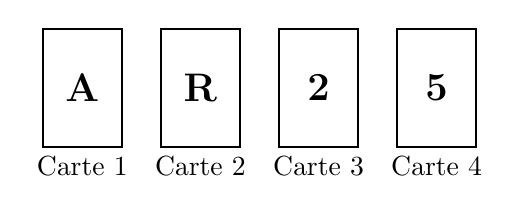
\begin{tikzpicture}[scale=0.5]
% Définition des styles
\tikzset{
card/.style={draw, thick, rectangle, minimum width=1cm, minimum height=1.5cm, align=center},
letter/.style={card},
number/.style={card}
}
% Carte A
\node[letter] at (0,0) {\Large \textbf{A}};
\node[below] at (0,-1.5) {Carte 1};
% Carte R
\node[letter] at (3,0) {\Large \textbf{R}};
\node[below] at (3,-1.5) {Carte 2};
% Carte 2
\node[number] at (6,0) {\Large \textbf{2}};
\node[below] at (6,-1.5) {Carte 3};
% Carte 5
\node[number] at (9,0) {\Large \textbf{5}};
\node[below] at (9,-1.5) {Carte 4};
\end{tikzpicture}
\end{center}
Alexandre affirme : \enquote{S'il y a une voyelle d'un côté d'une carte, alors il y a un chiffre pair de l'autre.}
Question : Quelles cartes faut-il retourner au minimum pour pouvoir vérifier si cette affirmation est vraie~?
\end{activite}

\section{Calcul littéral}
\begin{activite}
	\tcblower
	Traduire en expressions algébriques les données suivantes. La variable $x$ représente un nombre entier.
	\begin{tasks}
\task le carré d'un nombre impair;
\task un multiple de $n$;
\task trois nombres consécutifs quelconques; 
\task trois multiples de $17$ consécutifs;
\task le carré de la somme du produit de $2$ par $x$ et de $3$;
\task la différence des carrés de la différence du double de $x$ et de $5$ et de la somme de $x$ et de $3$;
\task le quadruple de la somme du centuple de l'unité et d'un nombre pair.
\end{tasks}
\end{activite}
\begin{activite}
	\tcblower
	\begin{tasks}
		\task On considère les conjectures suivantes où $n$ désigne un nombre entier naturel. Sont-elles vraies ou fausses~? Justifier.
		\begin{enumerate}
			    \item \textbf{Conjecture :} Si $n$ est un multiple de 9, alors $n$ est un multiple de 3.
    
    \item \textbf{Conjecture :} Si $n$ est un multiple de 3, alors $n$ est un multiple de 9.
    
    \item \textbf{Conjecture :} Le carré d'un nombre pair est toujours un nombre pair.
    
    \item \textbf{Conjecture :} Si $n^2$ est pair, alors $n$ est pair.
    
    \item \textbf{Conjecture :} $n^2$ est pair $\Leftrightarrow$ $n$ est pair.
    \item \textbf{Conjecture :} La somme de deux carrés est un carré. 
		\end{enumerate}
		\task Démontrer les assertations suivantes (qui sont toujours vraies). 
		\begin{enumerate}
			\item La somme de d'un nombre pairs et d'un nombre impair est un nombre impair. 
			\item Le produit de deux nombres impairs est un nombre impair.
			\item La somme de trois entiers consécutifs est un multiple de trois. 
		\end{enumerate}
	\end{tasks}
\end{activite}

\begin{activite}
	\tcblower
\end{activite}


\begin{activite}
	\tcblower
\end{activite}

\begin{activite}
	\tcblower
\begin{tasks}(1)
\task Qu'est-ce qu'une équation à une inconnue ?

\task Le nombre 3 est-il solution de l'équation $2x^2 + x = 1 - \dfrac{2}{5}x$ ?

\task Déterminer une équation de degré 1 dont l'ensemble de solution soit $S = \{2\}$

\task Déterminer une autre équation de degré 1 dont l'ensemble des solutions soit $S = \{2\}$

\task Ces deux équations sont-elles égales ?

\task Peut-on déterminer une équation de degré 1 dont l'ensemble des solutions soit $S = \emptyset$ ?
\end{tasks}
\end{activite}

\begin{activite}
	\tcblower
	\begin{tasks}
% --- Exercise 1 ---
\task Transformer chaque égalité en une égalité équivalente :

\vspace{0.5cm}
\begin{center}
\begin{tabular}{ccc}
% First row of diagrams
	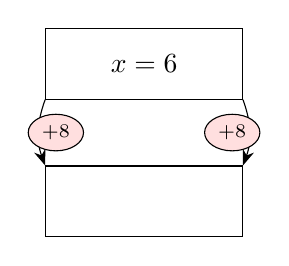
\begin{tikzpicture}[scale=0.7]
    \node[box] (top) at (0,0) {$x=6$};
    \node[box] (bottom) at (0,-2.5) {};
    \draw[-{Stealth[length=2mm]}] (top.200) to[out=-110,in=110] (bottom.160);
    \draw[-{Stealth[length=2mm]}] (top.-20) to[out=-70,in=70] (bottom.20);
\node[op] at (-1.6,-1.25) {\scriptsize$+8$};
    \node[op] at (1.6,-1.25) {\scriptsize$+8$};
\end{tikzpicture}
&
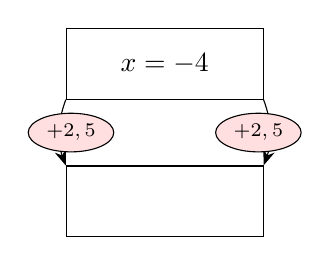
\begin{tikzpicture}[scale=0.7]

    \node[box] (top) at (0,0) {$x=-4$};
    \node[box] (bottom) at (0,-2.5) {};
    \draw[-{Stealth[length=2mm]}] (top.200) to[out=-110,in=110] (bottom.160);
    \draw[-{Stealth[length=2mm]}] (top.-20) to[out=-70,in=70] (bottom.20);
    \node[op] at (-1.7,-1.25) {\scriptsize$+2,5$};
    \node[op] at (1.7,-1.25) {\scriptsize$+2,5$};
\end{tikzpicture}
&
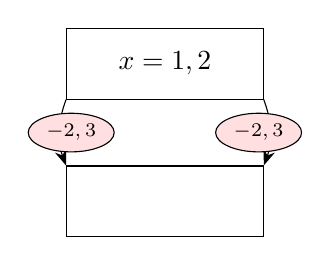
\begin{tikzpicture}[scale=0.7]

    \node[box] (top) at (0,0) {$x=1,2$};
    \node[box] (bottom) at (0,-2.5) {};
    \draw[-{Stealth[length=2mm]}] (top.200) to[out=-110,in=110] (bottom.160);
    \draw[-{Stealth[length=2mm]}] (top.-20) to[out=-70,in=70] (bottom.20);
    \node[op] at (-1.7,-1.25) {\scriptsize$-2,3$};
    \node[op] at (1.7,-1.25) {\scriptsize$-2,3$};
\end{tikzpicture}
\\ \\ \\
% Second row of diagrams
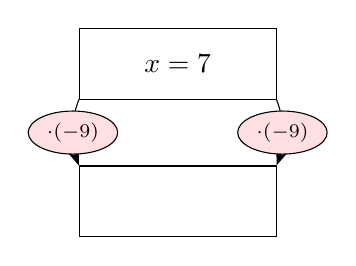
\begin{tikzpicture}[scale=0.7]

    \node[box] (top) at (0,0) {$x=7$};
    \node[box] (bottom) at (0,-2.5) {};
    \draw[-{Stealth[length=2mm]}] (top.200) to[out=-110,in=110] (bottom.160);
    \draw[-{Stealth[length=2mm]}] (top.-20) to[out=-70,in=70] (bottom.20);
    \node[op] at (-1.9,-1.25) {\scriptsize$\cdot(-9)$};
    \node[op] at (1.9,-1.25) {\scriptsize$\cdot(-9)$};
\end{tikzpicture}
&
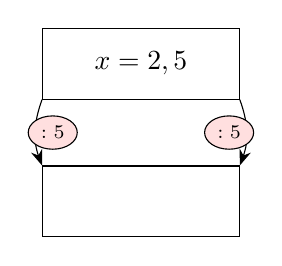
\begin{tikzpicture}[scale=0.7]

    \node[box] (top) at (0,0) {$x=2,5$};
    \node[box] (bottom) at (0,-2.5) {};
    \draw[-{Stealth[length=2mm]}] (top.200) to[out=-110,in=110] (bottom.160);
    \draw[-{Stealth[length=2mm]}] (top.-20) to[out=-70,in=70] (bottom.20);
    \node[op] at (-1.6,-1.25) {\scriptsize$: 5$};
    \node[op] at (1.6,-1.25) {\scriptsize$: 5$};
\end{tikzpicture}
&
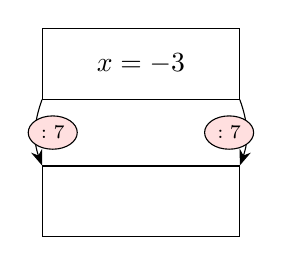
\begin{tikzpicture}[scale=0.7]

    \node[box] (top) at (0,0) {$x=-3$};
    \node[box] (bottom) at (0,-2.5) {};
    \draw[-{Stealth[length=2mm]}] (top.200) to[out=-110,in=110] (bottom.160);
    \draw[-{Stealth[length=2mm]}] (top.-20) to[out=-70,in=70] (bottom.20);
    \node[op] at (-1.6,-1.25) {\scriptsize$: 7$};
    \node[op] at (1.6,-1.25) {\scriptsize$: 7$};
\end{tikzpicture}
\end{tabular}
\end{center}

\vspace{0.5cm}
% --- Exercise 2 ---
\task Le but est de déterminer $x$ dans chacune des équations suivantes. Recopier puis déterminer $x$.

\vspace{1cm}

% First equation solving example
\noindent
\begin{minipage}[c]{0.20\linewidth}
\centering
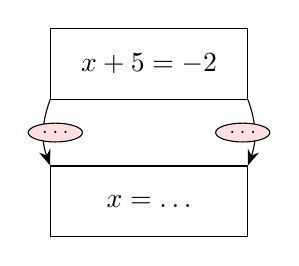
\begin{tikzpicture}[scale=0.7]
    \node[box] (top) at (0,0) {$x+5=-2$};
    \node[box] (bottom) at (0,-2.5) {$x = \dots$};
    \draw[-{Stealth[length=2mm]}] (top.200) to[out=-110,in=110] (bottom.160);
    \draw[-{Stealth[length=2mm]}] (top.-20) to[out=-70,in=70] (bottom.20);
    \node[op] at (-1.7,-1.25) {\scriptsize$\dots$};
    \node[op] at (1.7,-1.25) {\scriptsize$\dots$};
\end{tikzpicture}
\end{minipage}%
\begin{minipage}[c]{0.25\linewidth}
Rédaction :
\vspace{3cm}
\end{minipage}
% Second equation solving example
\begin{minipage}[c]{0.20\linewidth}
\centering
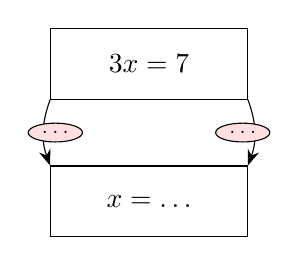
\begin{tikzpicture}[scale=0.7]
    \node[box] (top) at (0,0) {$3x=7$};
    \node[box] (bottom) at (0,-2.5) {$x = \dots$};
    \draw[-{Stealth[length=2mm]}] (top.200) to[out=-110,in=110] (bottom.160);
    \draw[-{Stealth[length=2mm]}] (top.-20) to[out=-70,in=70] (bottom.20);
    \node[op] at (-1.7,-1.25) {\scriptsize$\dots$};
    \node[op] at (1.7,-1.25) {\scriptsize$\dots$};
\end{tikzpicture}
\end{minipage}%
\begin{minipage}[c]{0.25\linewidth}
Rédaction :
\vspace{3cm}

\end{minipage}


\task Résoudre les équations suivantes en rédigeant comme ci-dessus. Vérifier ensuite que la solution est juste :

\begin{multicols}{3}
\begin{enumerate}
\item $x - 5,2 = 2,6$
\item $-6,5x = -14,2$
\item $-x = 7,2$
\end{enumerate}
\end{multicols}

\task De la même façon mais en deux étapes, résoudre les équations suivantes :

\begin{multicols}{2}
\begin{enumerate}
\item $2x + 3 = 4x + 7$

\item $7x - 6 = -1 + \dfrac{14x - 8}{2}$

\item $2,6 - 5x = -1,4$

\item $3(x+1) = x+2+2x+1$

\item $\dfrac{2}{3}x - \dfrac{1}{9} = \dfrac{3}{9}x + \dfrac{4}{2}$
\end{enumerate}
\end{multicols}
\end{tasks}
\end{activite}

\begin{activite}
	\tcblower
Voici l'énoncé du problème \enquote{somme-produit}:
\begin{quote}
\enquote{Déterminer deux nombres entiers $a$ et $b$ connaissant leur somme $S$ et leur produit $P$.} 
\end{quote}
Ce problème remonte aux babyloniens qui souhaitaient déterminer la longueur $\ell$ et la largeur $L$ d'un terrain rectangulaire (jardin, champ, etc.) connaissant son périmètre $2(\ell+L)$ et son aire $\ell\cdot L$. 

\begin{tasks}
\task Déterminer deux nombres $u$ et $v$ dont~:
\begin{multicols}{2}
	\begin{enumerate}
\item le produit vaut $6$ et la somme $5$

$u=\ligne{2}$ $v=\ligne{2}$
\item le produit vaut $12$ et la somme $7$

$u=\ligne{2}$ $v=\ligne{2}$
\item le produit vaut $12$ et la somme $-7$

$u=\ligne{2}$ $v=\ligne{2}$
\item le produit vaut $-5$ et la somme $4$

$u=\ligne{2}$ $v=\ligne{2}$
\item le produit vaut $10$ et la somme $-7$

$u=\ligne{2}$ $v=\ligne{2}$
\item le produit vaut $-9$ et la somme $8$

$u=\ligne{2}$ $v=\ligne{2}$
\item le produit vaut $-8$ et la somme $-2$

$u=\ligne{2}$ $v=\ligne{2}$
\item le produit vaut $15$ et la somme $-8$

$u=\ligne{2}$ $v=\ligne{2}$
\end{enumerate}
\end{multicols}

\task Écrire clairement une procédure pour obtenir une solution.  

	\vspace{15pt}
	\myrulefill
	\vspace{15pt}

	\myrulefill
	\vspace{15pt}

	\myrulefill

	\vspace{15pt}
\end{tasks}
Pour rappel, la quatrième identité remarquable est de la forme
\[(x+u)(x+v)=x^2+(u+v)x+uv.\]
On retrouve le terme somme ($u+v$) et le terme produit $uv$.
\begin{tasks}
	\task[c)] À l'aide du premier point, factoriser les expressions suivantes en utilisant la quatrième identité remarquable.
\begin{multicols}{2}
\begin{enumerate}
\item $x^2+5x+6=\ligne{4}$ 
\item $x^2+7x+12=\ligne{4}$
\item $x^2-7x+12=\ligne{4}$
\item $x^2+4x+-5=\ligne{4}$
\item $x^2-7x+10=\ligne{4}$
\item $x^2+8x-9=\ligne{4}$
\item $x^2-2x-8=\ligne{4}$
\item $x^2-8x+15=\ligne{4}$
\end{enumerate}
\end{multicols}

Un exemple de procédure. On note $P$ le produit et $S$ la somme. 
\tikzstyle{startstop} = [rectangle, rounded corners, minimum width=3cm, minimum height=1cm,text centered, draw=black,
execute at begin node={\begin{varwidth}{15em}},
execute at end node={\end{varwidth}}]
\tikzstyle{io} = [trapezium, trapezium left angle=70, trapezium right angle=110, minimum width=3cm, minimum height=1cm, text centered, draw=black, fill=blue!30]
\tikzstyle{process} = [rectangle, minimum width=3cm, minimum height=1cm, text centered, draw=black, fill=orange!30]
\tikzstyle{decision} = [diamond, minimum width=3cm, minimum height=1cm, text centered, draw=black, fill=green!30]
\tikzstyle{arrow} = [thick,->,>=stealth]
\begin{center}
\begin{tikzpicture}[scale=0.8,node distance=1.5cm]
	\node (e1) [startstop] {\centerline{Déterminer les diviseurs de $P$}};
	\node (e21) [startstop, below of=e1,  xshift=-6cm, yshift=-1cm] {\centerline{$P$ est positif~?}};
\node (e23) [startstop, below of=e1,  xshift=6cm, yshift=-1cm] {\centerline{$P$ négatif~?}};
\node (e34) [startstop, below of=e23, yshift=-1cm, xshift=0.5cm] {\centerline{$S$ positif}\centerline{$|u|\geq |v|$}\centerline{$u\geq0$ et $v\leq0$}};
\node (e31) [startstop, below of=e21, yshift=-1cm,xshift=-0.5cm] {\centerline{$S$ négatif}\centerline{$u\leq0$ et $v\leq0$}};
\node (e32) [startstop, below of=e21, xshift=3.5cm, yshift=-1cm] {\centerline{$S$ positif}\centerline{$u\geq0$ et $v\geq0$}};
\node (e33) [startstop, below of=e23, xshift=-3.5cm, yshift=-1cm] {\centerline{$S$ négatif}\centerline{$|u|\geq |v|$}\centerline{$u\leq0$ et $v\geq0$}};
\draw[arrow] (e1)--(e21);
\draw[arrow] (e1)--(e23);
\draw[arrow] (e21)--(e31);
\draw[arrow] (e21)--(e32);
\draw[arrow] (e23)--(e34);
\draw[arrow] (e23)--(e33);
\end{tikzpicture}
\end{center}

	Utiliser votre méthode ou la méthode ci-dessus pour déterminer deux nombres $u$ et $v$ dont~:
	\begin{multicols}{2}
	\begin{enumerate}
\item le produit vaut $-20$ et la somme $-8$

\vspace{15pt}
$u=\ligne{2}$ $v=\ligne{2}$
\item le produit vaut $-20$ et la somme $1$

\vspace{15pt}
$u=\ligne{2}$ $v=\ligne{2}$
\item le produit vaut $12$ et la somme $8$

\vspace{15pt}
$u=\ligne{2}$ $v=\ligne{2}$
\item le produit vaut $12$ et la somme $13$

\vspace{15pt}
$u=\ligne{2}$ $v=\ligne{2}$
\item le produit vaut $-40$ et la somme $3$

\vspace{15pt}
$u=\ligne{2}$ $v=\ligne{2}$
\item le produit vaut $28$ et la somme $-11$

\vspace{15pt}
$u=\ligne{2}$ $v=\ligne{2}$
	
\end{enumerate}
\end{multicols}
\task[d)] Factoriser à l'aide de la quatrième identité remarquable.
	\begin{multicols}{2}
	\begin{enumerate}
\item $x^2-8x-20=\ligne{4}$
\item $x^2+x-20=\ligne{4}$
\item $x^2-8x+12=\ligne{4}$
\item $x^2+13x+12=\ligne{4}$
\item $x^2+3x-40=\ligne{4}$
\item $x^2-11x+28=\ligne{4}$	
\end{enumerate}
\end{multicols}
\task[e)] Essayer de déterminer deux nombres $a$ et $b$ dont \[\text{le produit vaut } 233543149332 \text{ et la somme vaut } 1423373.\]
Si vous n'y arrivez pas, quel est l'obstacle rencontré par rapport à votre méthode ou à la méthode proposée~?

	\vspace{15pt}
	\myrulefill
	\vspace{15pt}

	\myrulefill
	\vspace{15pt}

	\myrulefill
	\vspace{15pt}


	\myrulefill
	\vspace{15pt}


\end{tasks}
\end{activite}
\begin{activite}
	\tcblower
	\begin{tasks}
		\task Résoudre les équations suivantes

		\begin{center}	
		\begin{inlineumerate}
		\item $2x+1=3$\hspace{3cm}
		\item $3x+1=3$
		\end{inlineumerate}
		\end{center}
\task Résoudre l'équation avec paramètre $a$ pour l'inconnue $x$~ 
\[ax+1=3.\]
\vspace{-0.8cm}
\task Résoudre l'équation avec paramètre $a$ pour l'inconnue $x$~: \[x+3a=2x+1\]
\vspace{-0.8cm}
\task Résoudre l'équation avec paramètre $a$ pour l'inconnue $x$~:\[2x-4=ax+3.\]
\vspace{-0.8cm}
\task Que remarquez-vous~?
	\end{tasks}
\end{activite}
\newpage
\section{Équations}
\begin{activite}
	\tcblower
	Voici neuf énoncés et onze équations. Chaque énoncé correspond à une des équations proposées. Retrouver laquelle et justifier.
	Poser à chaque fois l'inconnue $x$.
\vspace{5pt}

\begin{tabularx}{\textwidth}{|c|X|c|}
	\hline 1 & Une balance à deux plateaux est en équilibre lorsque l'on place 10 cubes et une masse de 2 kg sur l'un des plateaux et 2 cubes et une masse de 30 kg sur l'autre. Quelle est la masse d'un cube? & \phantom{22}\\
\hline 2 & Une troupe théâtrale donne une représentation au collège. Pour payer le cachet des acteurs, chaque élève doit payer 30 Fr. Le jour de la représentation, 10 élèves sont absents, et chaque élève doit payer 2 Fr. de plus que prévu. Combien d'élèves assistent à cette représentation?& \phantom{22} \\
\hline 3 & Un père a 30 ans et son fils a 10 ans. Dans combien d'années l'âge du père sera-t-il le double de celui du fils? & \phantom{22}\\
\hline 4 & Pour aller de Grenoble au col du Lautaret, un touriste à vélo roule à la vitesse de $10 \mathrm{~km} / \mathrm{h}$. Il se repose 2 heures au col du Lautaret. Au retour, il roule à la vitesse de $30 \mathrm{~km} / \mathrm{h}$. Sachant que cet entraînement a duré 10 heures, quelle est la distance séparant Grenoble du col du Lautaret? & \phantom{22}\\
\hline 5 & Un rectangle est tel que sa longueur est le double de sa largeur. Si on augmente sa longueur de 30 m et si on diminue sa largeur de 10 m , son aire est multipliée par 2. Quelle est la largeur initiale du rectangle? & \phantom{22}\\
\hline 6 & Un pavé droit a une hauteur de 30 cm ; sa largeur est le dixième de sa longueur et lorsque l'on calcule l'aire totale et le volume de ce pavé, on trouve les mêmes nombres (l'un en $\mathrm{cm}^2$ et l'autre en $\mathrm{cm}^3$). Quelle est la largeur de ce pavé? & \phantom{22}\\
\hline 7 & L'eau de Javel est utilisée diluée. Une solution diluée à 2\% contient 2 cl d'eau de Javel et 98 cl d'eau pour former un litre (100 cl) de solution. Une solution diluée à $30 \%$ contient 30 cl d'eau de Javel pour former un litre (100 cl) de solution. Quelle quantité de solution à $30 \%$ faut-il ajouter à 1 litre d'une solution à $2 \%$ pour obtenir une solution à $10 \%$ ? & \phantom{22}\\
\hline 8 & On dispose d'une plaque de carton carrée de 10 cm de côté. On découpe quatre carrés (un dans chaque coin) et on plie de façon à obtenir une boîte sans couvercle. Quelle est la dimension des carrés à découper pour que le volume de la boîte soit égal à $30 \mathrm{~cm}^3$ ? & \phantom{22}\\
\hline 9 & Un arbre haut de 10 m et un poteau haut de 2 m sont situés en face l'un de l'autre sur chacune des rives d'une rivière large de 30 m . Au sommet de chacun d'eux est perché un oiseau. Ils se lancent tous deux à la même vitesse et au même instant sur une pauvre mouche qui les nargue à la surface de l'eau. Par un effet magique de Dame Nature, ils l'atteignent au même moment et se fracassent le bec dans un contact plus que vigoureux, et de ce fait se retrouvent bredouilles. A quelle distance du pied de l'arbre se trouvait cette mouche miraculée? & \phantom{22}\\
\hline
\end{tabularx}

\vspace{5pt}

\begin{tasks}(3)
\task $\dfrac{x}{10}+2+\dfrac{x}{30}=10$
\task $10(x+2)=30 x$
\task $x(10-2 x)(10-2 x)=30$
\task $(30+x)=2(10+x)$
\task $30(x+10)=x(30+2)$
\task $\dfrac{30 x}{2}+\dfrac{10 x}{2}=\dfrac{1}{2}(x+10) 30$
\task $10 x+2=2 x+30$
\task $x^2+10^2=(30-x)^2+2^2$
\task $(2 x+30)(x-10)=2 x(2 x)$
\task $\dfrac{30}{100} x+\dfrac{2}{100}=(x+1) \dfrac{10}{100}$
\task*(2) $2(30 x+x \cdot 10 x+30 \cdot 10 x)=x \cdot 10 x \cdot 30$
\end{tasks}

\end{activite}
\begin{activite}
	\tcblower
	\begin{tasks}
   \task Un magasin de vêtements faisant les soldes annonce que tous les prix ont été baissés de 20\%. Si le prix d'une chemise soldée est 28.- quel était son prix de vente ?
    \task Le sixième d'un piquet est enfoncé dans la terre, les deux cinquièmes dans la neige et le reste, qui est en dehors, mesure 3,25m. La température de l'air est de 4°C. Trouver la hauteur du piquet.
    \task Une société d'investissement a 100'000.- à investir pour un client et décide d'investir dans deux fonds, A et B. L'intérêt annuel attendu pour le fonds A est de 15\%, mais il y a un certain risque et le client ne veut pas investir plus de 50'000.- dans ce fonds. Pour le fonds B, plus solide, l'intérêt est de 10\%. Déterminer s'il y a une façon d'investir l'argent pour que l'intérêt annuel soit :
    
    \begin{center}
    \begin{inlineumerate}
    \item 12'000.-\hspace{3cm}
        \item 13'000.-
    \end{inlineumerate}
\end{center}
\end{tasks}
\end{activite}

\begin{activite}
 Il s'agit, avec la calculatrice, d'être le plus efficace et précis possible pour effectuer les calculs demandés (en utilisant si besoin des parenthèses ou si nécessaire). Pour chaque calcul, donnez être capable de décrire précisément (par exemple en donnant la suite de touches utilisée) la façon dont la calculatrice a été utilisée.

\begin{tasks}
\task Calculer à l'aide de la calculatrice la valeur arrondie au millième de :
\begin{multicols}{3}	
\begin{enumerate}
\item $4 \cdot (2 + 3)$
\item $3 \cdot \pi$
\item le quart de la réponse précédente
\item $4\pi$ au carré
\item $2 : 5$
\item $0,25 \cdot 0,5$
\item $-325,201569 - 2,82589$
\item $5 \cdot \sqrt{4}$
\item $\dfrac{4,7 : (6,76 - 0,95)}{5,001}$
\end{enumerate}
\end{multicols}

\task Effectuer les calculs suivants en utilisant l'écriture scientifique de la calculatrice :

\begin{inlineumerate}
\item $(7,28 \cdot 10^{13}) \cdot 10^5$
\item $(-7,28 \cdot 10^{-8}) : 3 \cdot 10^4$
\end{inlineumerate}

\task Simplifier le plus possible $\dfrac{49005}{6030}$ à l'aide de la calculatrice.

\task Calculer $\dfrac{2}{35}$ puis $\dfrac{2}{3} \cdot 5$
\end{tasks}
\end{activite}
\end{document}
